\documentclass[UTF8]{ctexart}
\usepackage{tikz}
\begin{document}
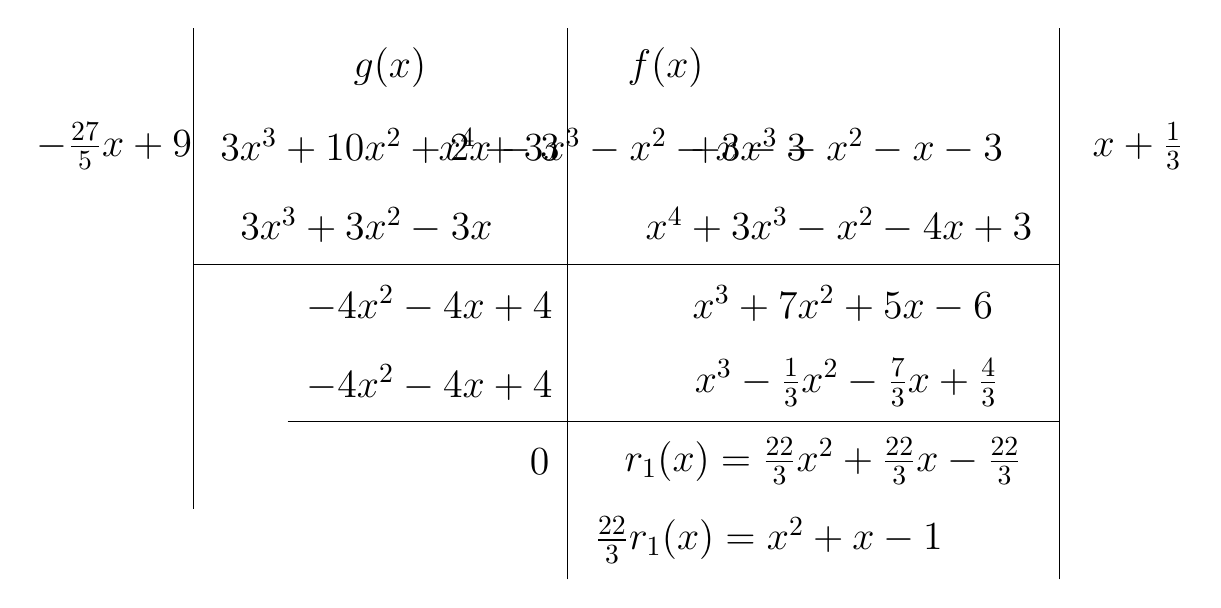
\begin{tikzpicture}
  \path (-4,2) node[font=\Large] {$-\frac{27}{5}x+9$};
  \path (3,3) node[font=\Large] {$f(x)$};
  \path (2.45,2) node[font=\Large] {$x^4+3x^3-x^2-x-3$};
  \path (5.3,2) node[font=\Large] {$ +3x^3-x^2-x-3$};
  \path (5.2,1) node[font=\Large] {$x^4+3x^3-x^2-4x+3$};
  \path (5.25,0) node[font=\Large] {$x^3+7x^2+5x-6$};
  \path (5.3,-1) node[font=\Large] {$x^3-\frac13 x^2-\frac73 x+\frac43$};
  \path (5,-2) node[font=\Large] {$r_1(x)=\frac{22}{3} x^2+\frac{22}{3} x-\frac{22}{3}$};
  \path (4.31,-3) node[font=\Large] {$\frac{22}{3} r_1(x)=x^2+x-1$};
  \path (-0.5,3) node[font=\Large] {$g(x)$};
  \path (-0.5,2) node[font=\Large] {$3x^3+10x^2+2x-3$};
  \path (-0.8,1) node[font=\Large] {$3x^3+3x^2-3x$};
  \path (9,2) node[font=\Large] {$x+\frac13$};
  \path (0,0) node[font=\Large] {$-4x^2-4x+4$};
  \path (0,-1) node[font=\Large] {$-4x^2-4x+4$};
  \path (1.4,-2) node[font=\Large] {$0$};
  \draw (1.75,-3.5) -- (1.75,3.5);
  \draw (-3,-2.6) -- (-3,3.5);
  \draw (8,-3.5) -- (8,3.5);
  \draw (-3,0.5) -- (8,0.5);
  \draw (-1.8,-1.5) -- (8,-1.5);
\end{tikzpicture}
\end{document}

